\section{Spectral Burrows Wheeler Transform}\label{sec:SBWT}

Succinct data structures are those which represent the necessary data close to its information-theoretic bound while still allowing fast searches within it~\cite{Succinct}.
The Spectral Burrows Wheeler Transform (SBWT)~\cite{SBWT} represents the DBG as a succinct data structure.
In this case, it represents it as a collection of bit vectors.
The first to do this were the authors of BOSS~\cite{SuccinctDeBruijnGraphs}, but the authors of SBWT managed to create a data structure where searching for the index of a $k$-mer takes $O(k)$~\cite{SBWT}.
In this section, the construction of this structure is discussed, as well as how to use it, and its limitations.
One limitation will be mentioned now to make sure the reader does not get confused while reading.
This data structure only guarantees searches for $k$-mers of fixed size.
This means that if the data structure was built with $k=31$, then it will only support queries for $k$-mers of size $k=31$ or less.

\subsection{Construction}

In this subsection an SBWT structure will be built.
Although the name implies that a Burrows Wheeler Transform (BWT)~\cite{BWT} is used for this succinct data structure, the similarities are distant enough that it is possible to explain the SBWT without going into details of the BWT.\@
Figure~\ref{fig:SbwtConstruction} shows the entire construction pipeline in a single figure, so it is good to refer to it while reading the rest of this section.
The first step is to extract all $k$-mers and reverse complements and create a DBG where an edge $a \rightarrow b$ is drawn for every $k$-mer $a$ and $b$ where the $k-1$ suffix of $a$ is equal to the $k-1$ prefix of $b$.
For example, given $k=3$ and the $k$-mers \textit{ACG, CGA}, and \textit{CGT}, edges $ACG \rightarrow CGA$ and $ACG \rightarrow CGT$ are created, because the $k-1=2$ suffix of \textit{ACG} is equal to the $k-1=2$ prefix of the other two $k$-mers.
The necessary $\$$ $k$-mers are then added to this DBG.\@

Next, the $k$-mers are sorted in ascending colexicographic order.
Colexicographic order means that to get the weight of the string, the reverse of the string must be considered.
After reversing, the  strings can then be sorted in ascending lexicographic/alphabetic order.
The $\$$ character is always weighted as smaller than all the other characters when sorting, meaning that the alphabet, in ascending order, is $\$ACGT$.

From the DBG, the labels of the outgoing edges are extracted and associated with the sorted $k$-mers.
These are then collapsed, such that only the first $k$-mer with a unique suffix of size $k-1$ has outgoing edges.
The collapse is a union, or, since edges with the same $k-1$ suffix will always have the same outgoing edges due to the DBG construction step, one can simply set the outgoing edge label set of the other nodes as the empty set $\emptyset$.
After collapsing, the edge labels column can be replaced with 4 bitvectors, one for each character.
Notice that no edge can ever have a $\$$ symbol, so there is no need for 5 bitvectors, even though the alphabet size is 5.
A cumulative sum map is also created, which is labeled as the c-map.
This stores the cumulative sum of the bit vectors, starting from 1 and then adding up each bit vector for each letter in ascending order.

\begin{figure}[t]
  \centering
  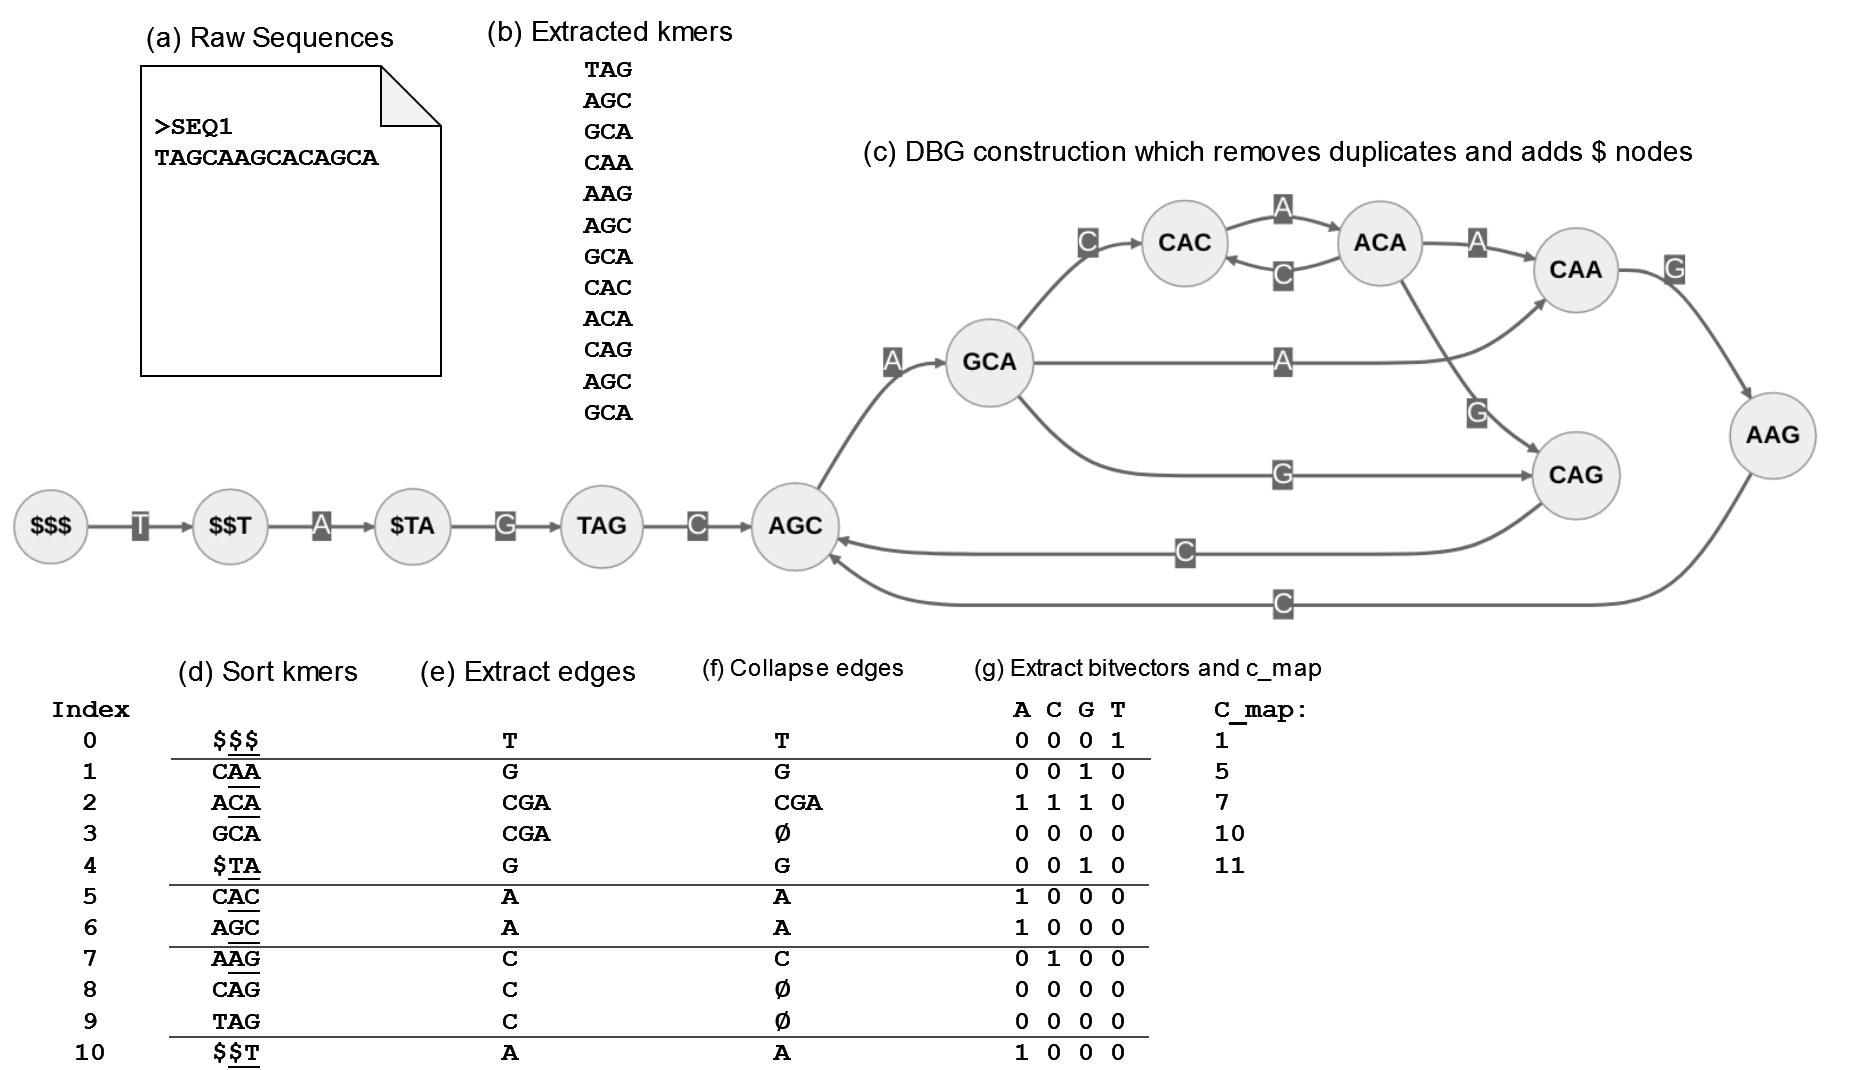
\includegraphics[width=\textwidth]{images/SbwtConstruction.png}
  \caption{SBWT construction pipeline. Note that for this example, the reverse complements are omitted for simplicity and clarity. The first edge is underlined in the sorted lists with unique $k-1$ prefixes.}\label{fig:SbwtConstruction}
\end{figure}

\subsection{Querying}\label{sec:SBWTQuerying}

For querying, one can use a technique similar to a BWT query~\cite{BWT}.
Remember that the only queries which can be done are for $k$-mers of size $k$ or less, that is, the same $k$ used in construction.
The notation will first be defined informally with an informal traversal example, before formally defining the efficient algorithm for traversal.

For the examples, the same construction from Figure~\ref{fig:SbwtConstruction} will be used.
In this figure, long gray lines indicate where the $k$-mers associated with one character begins and where those associated with the previous character ends in the sorted list.
Let $k$-mers associated with a character $c$ mean that the last character of the $k$-mer is $c$.
The list of $k$-mers associated with a character $c$ is $K_c = [k_1, k_2, \ldots, k_{c_{\max}}]$.
To search, two pointers are kept track of, a \textit{left} pointer and a \textit{right} pointer.
In the context of the figure, left means top, and right means bottom.
The algorithm shifts these two pointers around until they meet if the $k$-mers exist, or until the left pointer is greater than the right pointer, in which case it means that the $k$-mer was not found.
These pointers are concerned with the collapsed edges list, so look at these while going through the example.
The informal pseudo code is given in Algorithm~\ref{alg:IndexSearchInformalPseudoCode}, and the formal pseudo code will be discussed next and is then summarised by Algorithm~\ref{alg:IndexSearchFormalPseudoCode}.

\begin{algorithm}
	\KwIn{\newline
    A sequence $S = c_1, c_2, \ldots, c_k$ \newline
    The list of collapsed edges \newline
		The list of indexes where each $k$-mer set associated with one character starts and ends\newline
	}
	$\mathit{left}$ = index of first $k$-mer associated with $c_1$

	$\mathit{right}$ = index of last $k$-mer associated with $c_1$

	\ForEach{c \textbf{in} S[2 \ldots $k$]}{
    $\mathit{left}$ = index of first $k$-mer associated with $c$ + number of characters $c$ up to this pointer in the collapsed edges list ($\mathit{left}$), the index of this pointer not included

    $\mathit{right}$ = index of first $k$-mer associated with $c$ + number of characters $c$ up to this pointer in the collapsed edges list ($\mathit{right}$), the index of this pointer included \-- 1

    \If{$\mathit{left}$ > $\mathit{right}$}{\
      \textbf{return} not found
    }
  }
  \textbf{return} $\mathit{left}$ \textit{// or }$\mathit{right}$\textit{, they will have the same value}
	\caption{Index Search function (Informally Defined)}\label{alg:IndexSearchInformalPseudoCode}
\end{algorithm}

This next part will go through a full example search for the sequence $\mathit{CAC}$, which is know to exist in the dataset.
While doing this example, the reader is invited to look at Figure~\ref{fig:IndexQueryExample} for a visual representation of the movement of the left and right pointers.
The first character is $C$, so the algorithm starts by placing the pointers at the start and end of the $k$-mers associated with the character $C$, that is, indexes 5 and 6 for the left and right pointers respectively.
The next character is $A$, so the algorithm performs a check for how many $A$s there are in the collapsed edges list, until it gets to each of the left and right pointers, with the exception that for the left pointer, the $A$ at the index of this pointer itself is not included.
Thus, for the left pointer, the algorithm has a single $A$, so it moves the left pointer to the index of the $k$-mer associated with the first $A$ + 1, that is, index 2.
At index 6, including the index itself, it has three $A$s, so it moves this pointer to the index of the $k$-mer associated with the first $A$ + 3, that is, index 3.
Lastly, the right pointer must be moved one index downwards, so now it is at index 2, same as the left pointer.

\begin{figure}[t]
  \centering
  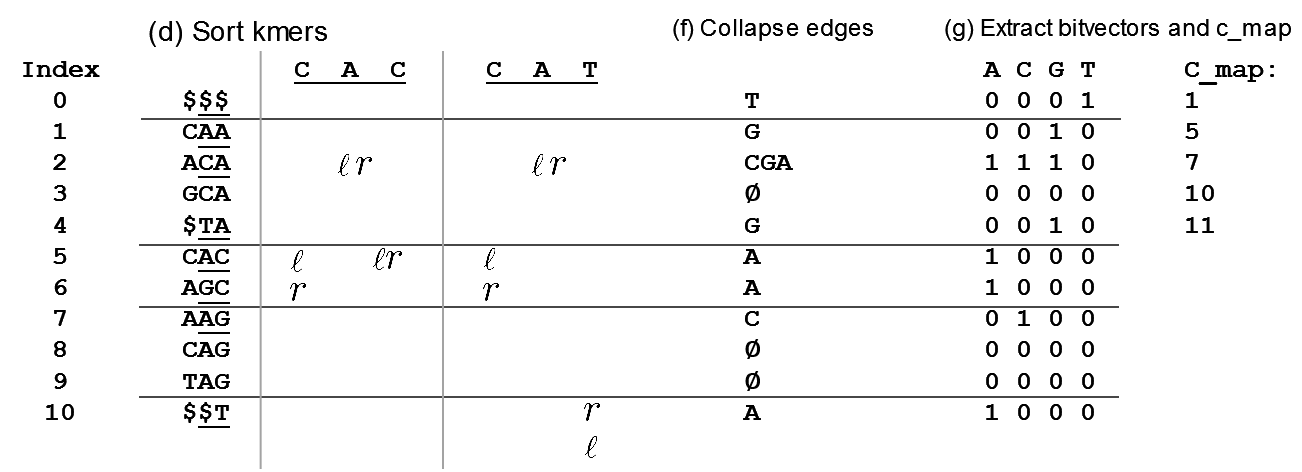
\includegraphics[width=\textwidth]{images/IndexQueryExample.png}
  \caption{Two examples of querying through the SBWT structure created in Figure~\ref{fig:SbwtConstruction}. The sequences $CAC$ is searched, which is found, and $CAT$ is not found.}\label{fig:IndexQueryExample}
\end{figure}

Lastly is the character $C$ again.
At the left pointer, up to this point there have been no $C$s in the collapsed edge list, so the pointer is moved to the index of the $k$-mer associated with the first $C$, that is, index 5.
Including the index at the right pointer, a single $C$ has been seen, so the pointer is moved to the index of the first $C$ + 1, to index 6, and then move one index backwards, to index 5.
The algorithm has now reached the end of the string, and the left and right pointer are equal and are both at index 5, which means that the index of the $k$-mer $CAC$ in the SBWT is 5.
By looking at the sorted $k$-mer list again, this claim may be verified.
The reader is encouraged to try this with other $k$-mers as well.

In the end of a $k$-mer query, the left and right pointer will always be equal, if the $k$-mer has been found.
This works because the $k$-mers are sorted and the edges are collapsed.
When the edges are collapsed, the algorithm is essentially making sure that in the DBG, each edge only has a single incoming node~\cite{SBWT}, as seen in Figure~\ref{fig:PrunedDBG}.
Next is an example using the same technique, but for a $k$-mer not present in the dataset.

\begin{figure}[t]
  \centering
  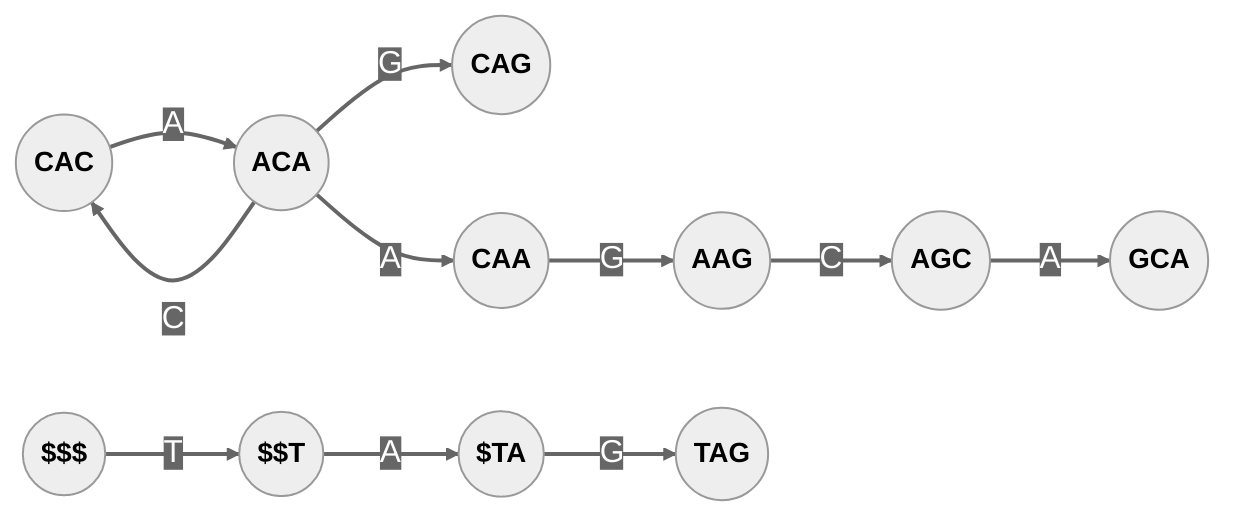
\includegraphics[width=\textwidth]{images/PrunedDbg.png}
  \caption{Pruned DBG from figure~\ref{fig:SbwtConstruction}}\label{fig:PrunedDBG}
\end{figure}

Now the sequence $\mathit{CAT}$ is considered.
Following from the previous example, both of the pointers will be at index 2 after considering both characters C and A.
Now put the left pointer at the index associated with the first $T$ + the number of $T$s seen thus far, which is $10 + 1 = 11$.
Similarly, the right pointer is put in the same location \-- 1, that is, at index 10.
Now, the left pointer is greater than the right pointer, so the algorithm will return that the $k$-mer has not been found.
Figure~\ref{fig:IndexQueryExample} also shows this example visually.

Now comes the definition for how one can do these queries algorithmically and in an efficient manner.
Notice that by using the c-map, one can know where the first $k$-mer associated with each character is.
The first element of this map is always 1, due to the node containing $k$ $\$$s.
Then, using the bitvectors for each character, the number of characters that exist up to that point in the collapsed edge list can be known, by counting the number of 1s.
To count the number of 1s, the algorithm uses what is known as the rank function for bitvectors.
Thus, $rank(b, i)$ gives the number of 1s for the bitvector $b$  up to but not including the index $i$.
For example, given $b=010110$ in binary, $rank(b, 0) = 0, rank(b, 1) = 0, rank(b, 2) = 1, rank(b, 3) = 1, rank(b, 4) = 2, rank(b, 5) = 3$ and $rank(b, 6) = 3$.
The formal definition of the algorithm can be now seen in Algorithm~\ref{alg:IndexSearchFormalPseudoCode}.

\begin{algorithm}
	\KwIn{\newline
    A sequence $S = c_1, c_2, \ldots, c_k$ \newline
    Bitvectors $b_A, b_C, b_G, b_T$
    c-map $C$
	}
  $\mathit{left}$ = $C[c]$

  $right$ = $C[c+1]$\--1  \textit{// C[A] = C[0], C[C] = C[1], \ldots}

	\ForEach{c \textbf{in} S[2 \ldots $k$]}{
    $\mathit{left}$ = $C[c]$ + rank ($b_c$, $\mathit{left}$)

    $right$ = $C[c]$ + rank ($b_c$, $\mathit{right} + 1$) \-- 1

    \If{$\mathit{left}$ > $\mathit{right}$} {\
      \textbf{return} not found
    }
  }
  \textbf{return} $\mathit{left}$
  \caption{Index Search function (Formally Defined)}\label{alg:IndexSearchFormalPseudoCode}
\end{algorithm}

Note that since $i$ itself is not included, $\mathit{rank}(0) = 0$ always holds.
Some other material may define this rank function a bit differently, such as including the 1s at index $i$, however, in this thesis, it is defined this way in order to stay true to the implementation.
This is also the implementation used by $sdsl$~\cite{SDSL}, which is a popular bitvector manipulation library.
Knowing all this, one can view the c-map as a cache for cumulative bitvector sums (+1), which means that when storing the SBWT, only two items are needed: the bitvectors, and the value for $k$, as everything else can be recomputed.

The heaviest part of this algorithm is the rank function.
Counting the number of 1s from the start of the bitvector at each step would be extremely inefficient.
On the previous CPU implementation of Themisto~\cite{Themisto}, the SDSL~\cite{SDSL} rank function is used.
Meanwhile, on the previous GPU implementation~\cite{Harri}, the Poppy data structure~\cite{Poppy} is used, to turn the rank function from $O(n)$, where $n$ is the number of vertices in the DBG, to $O(1)$, needing at most 3 cache line accesses per query.
This makes the entire search function $O(k)$.
For this thesis, Poppy is used, hence this will be further focused on.
Another advantage of this data structure is that its memory footprint is negligible, as it only uses 6.25\% more memory than the bitvector alone~\cite{Poppy}.

To construct the Poppy data structure, the vectors can be scanned once and checkpoints are inserted at each step.
For those familiar with skip lists, the cost-saving ideas are comparable.
Checkpoints are set at 3 layers.
Layer 0 stores a checkpoint every $2^{32}$ bits, so that it counts the total cumulative number of bits.
This type of cumulativeness is called absolute cumulative.
Thus, $2^{32}$ is the hyperblock size.
Layer 0 is stored as a bitvector of 64-bit integers.

Next is to construct layer 1.
This layer is similar to to layer 0 but it stores a checkpoint after $2^{10} = 1024$ bits.
$2^{10}$ is the superblock size.
Another special feature of this layer is that it resets to 0 once it reaches one of the layer 0 checkpoints, that is, once the number of bits it has covered reaches the hyperblock size, it restarts from 0.
This gives it the feature that layer 1 counts will always have a maximum size of $2^{32}$, and thus can be stored in 32-bit integers.

Lastly is layer 2, which sets a checkpoint after every $2^8 = 256$ bits, or after every $4 \times 64$ bits.
$2^8$ is the basicblock size.
This layer is not cumulative at all, unlike the previous two layers, where layer 1 is relative cumulative and layer 0 is absolute cumulative.
The maximum value for layer 2 is $2^8$, which means that for each value, they only need 8 bits.
Layer 3 could be considered to be the bitvector itself.
The full data structure is shown in the first part of Figure~\ref{fig:Poppy}.

\begin{figure}[t]
  \centering
  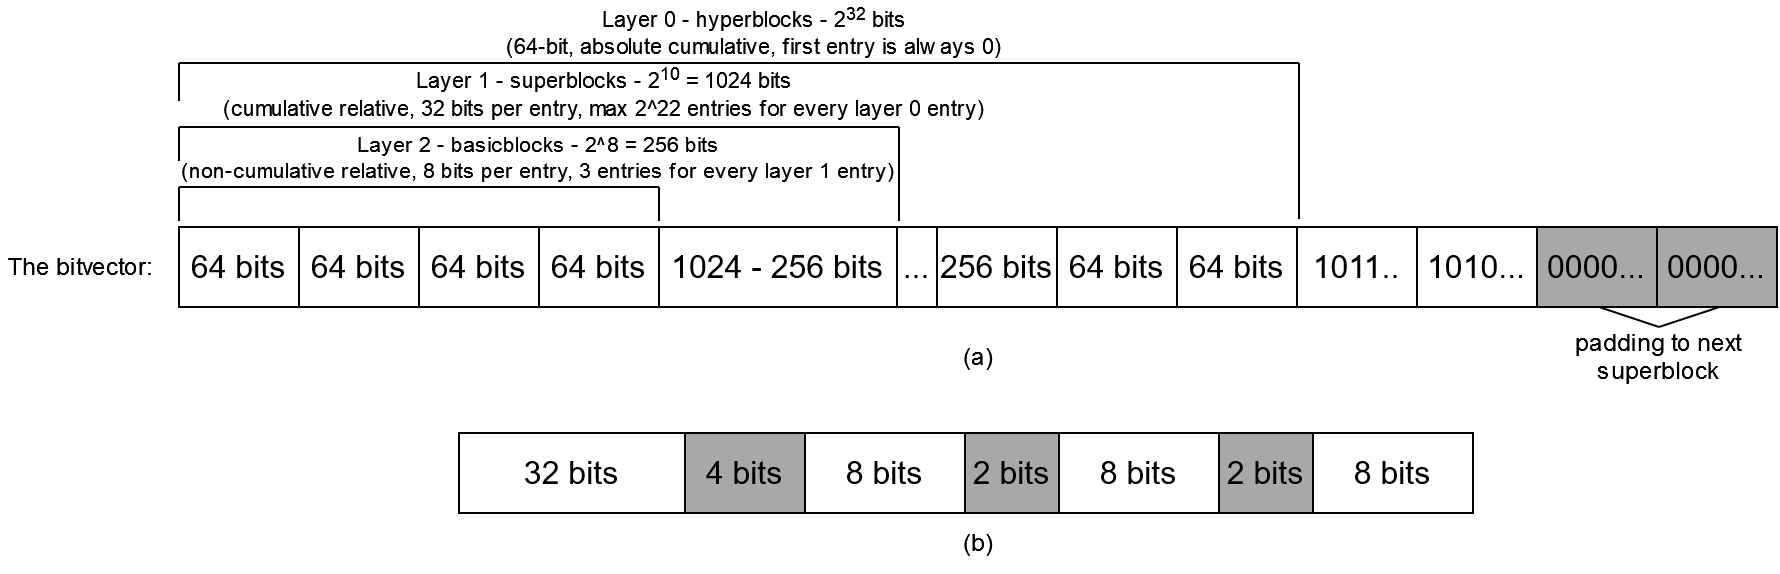
\includegraphics[width=\textwidth]{images/Poppy.png}
  \caption{(a) Poppy data structure fully constructed, with padding shown to the next superblock. (b) The combined storage representation for layer 1 and layer 2.}\label{fig:Poppy}
\end{figure}

Then, to query, one would need to first obtain the previous layer 0 entry, which always has a 0 entry at the start for convenience.
This entry is then added to the previous layer 1 entry, which also has a 0 entry at the start.
The result would then need be added to the previous layer 2 entries within the same superblock.
Lastly, the rank of the integers within the same basicblock is added up until the index needed for the rank function.

The storage of layers 1 and 2 can be combined in a single 64-bit integer, so the data structure can have a layer 1 entry and the inner layer 2 entries.
This is shown in the second part of Figure~\ref{fig:Poppy}.
As a result of this optimisation, the algorithm may need to do more bit shifting in order to obtain the values for layers 1 and 2, however the values in these layers can be accessed with a single memory access, which is usually a bigger bottleneck than bit shifts.
The big advantage of this data structure is that it can handle vectors up to $2^{64}$ bits, which is the maximum that the algorithm as a whole can handle.

This concludes the SBWT section.
Note, again, that this algorithm guaranteed to find $k$-mers of the size of the same $k$ with which the algorithm was built for, or less.
As such, $k$ should be as large as possible, if accuracy is the goal.
However, the larger the $k$, the larger the memory footprint of the index, so it is not recommended to go overboard.
$k=31$ is a usual choice, as the entire query can fit into a single 64-bit integer by bit packing ACGT into 2 bits each, though this technique is not used by the implementation for this thesis, which is in Section~\ref{sec:Phase1}.
$k$ is taken to be 31 since this is an odd number and palindromes should be avoided, as discussed earlier.
The disadvantage of this data structure is that information is lost as to where the $k$-mer originated from, if the input consists of multiple reads, or multiple files.
The next section will describe how additional labels, known as colors in this domain, can be added to the vertices in the DBG in order to determine where the $k$-mers originate from.
